\documentclass[portrait]{baposter}

\usepackage{times}
\usepackage{calc}
\usepackage{graphicx}
\usepackage{amsmath}
\usepackage{amssymb}
\usepackage{relsize}
\usepackage{multirow}
\usepackage{bm}
\usepackage{minted}
\usepackage{booktabs}

\usepackage{graphicx}
\usepackage{multicol}

\usepackage{pgfbaselayers}
\pgfdeclarelayer{background}
\pgfdeclarelayer{foreground}
\pgfsetlayers{background,main,foreground}

\newcommand{\captionfont}{\footnotesize}

\selectcolormodel{cmyk}

\graphicspath{{images/}}

%%%%%%%%%%%%%%%%%%%%%%%%%%%%%%%%%%%%%%%%%%%%%%%%%%%%%%%%%%%%%%%%%%%%%%%%%%%%%%%%
%%%% Some math symbols used in the text
%%%%%%%%%%%%%%%%%%%%%%%%%%%%%%%%%%%%%%%%%%%%%%%%%%%%%%%%%%%%%%%%%%%%%%%%%%%%%%%%

%%%%%%%%%%%%%%%%%%%%%%%%%%%%%%%%%%%%%%%%%%%%%%%%%%%%%%%%%%%%%%%%%%%%%%%%%%%%%%%%
% Multicol Settings
%%%%%%%%%%%%%%%%%%%%%%%%%%%%%%%%%%%%%%%%%%%%%%%%%%%%%%%%%%%%%%%%%%%%%%%%%%%%%%%%
\setlength{\columnsep}{0.5em}
\setlength{\columnseprule}{0mm}

%%%%%%%%%%%%%%%%%%%%%%%%%%%%%%%%%%%%%%%%%%%%%%%%%%%%%%%%%%%%%%%%%%%%%%%%%%%%%%%%
% Save space in lists. Use this after the opening of the list
%%%%%%%%%%%%%%%%%%%%%%%%%%%%%%%%%%%%%%%%%%%%%%%%%%%%%%%%%%%%%%%%%%%%%%%%%%%%%%%%
\newcommand{\compresslist}{
    \setlength{\itemsep}{1pt}
    \setlength{\parskip}{0pt}
    \setlength{\parsep}{0pt}
}

%%%%%%%%%%%%%%%%%%%%%%%%%%%%%%%%%%%%%%%%%%%%%%%%%%%%%%%%%%%%%%%%%%%%%%%%%%%%%%
%%% Begin of Document
%%%%%%%%%%%%%%%%%%%%%%%%%%%%%%%%%%%%%%%%%%%%%%%%%%%%%%%%%%%%%%%%%%%%%%%%%%%%%%

\begin{document}

%%%%%%%%%%%%%%%%%%%%%%%%%%%%%%%%%%%%%%%%%%%%%%%%%%%%%%%%%%%%%%%%%%%%%%%%%%%%%%
%%% Here starts the poster
%%%---------------------------------------------------------------------------
%%% Format it to your taste with the options
%%%%%%%%%%%%%%%%%%%%%%%%%%%%%%%%%%%%%%%%%%%%%%%%%%%%%%%%%%%%%%%%%%%%%%%%%%%%%%
\typeout{Poster Starts}
\background{
  \begin{tikzpicture}[remember picture,overlay]
    \draw (current page.north west)+(-2em,-0em) node[anchor=north west] {\hspace{-2em}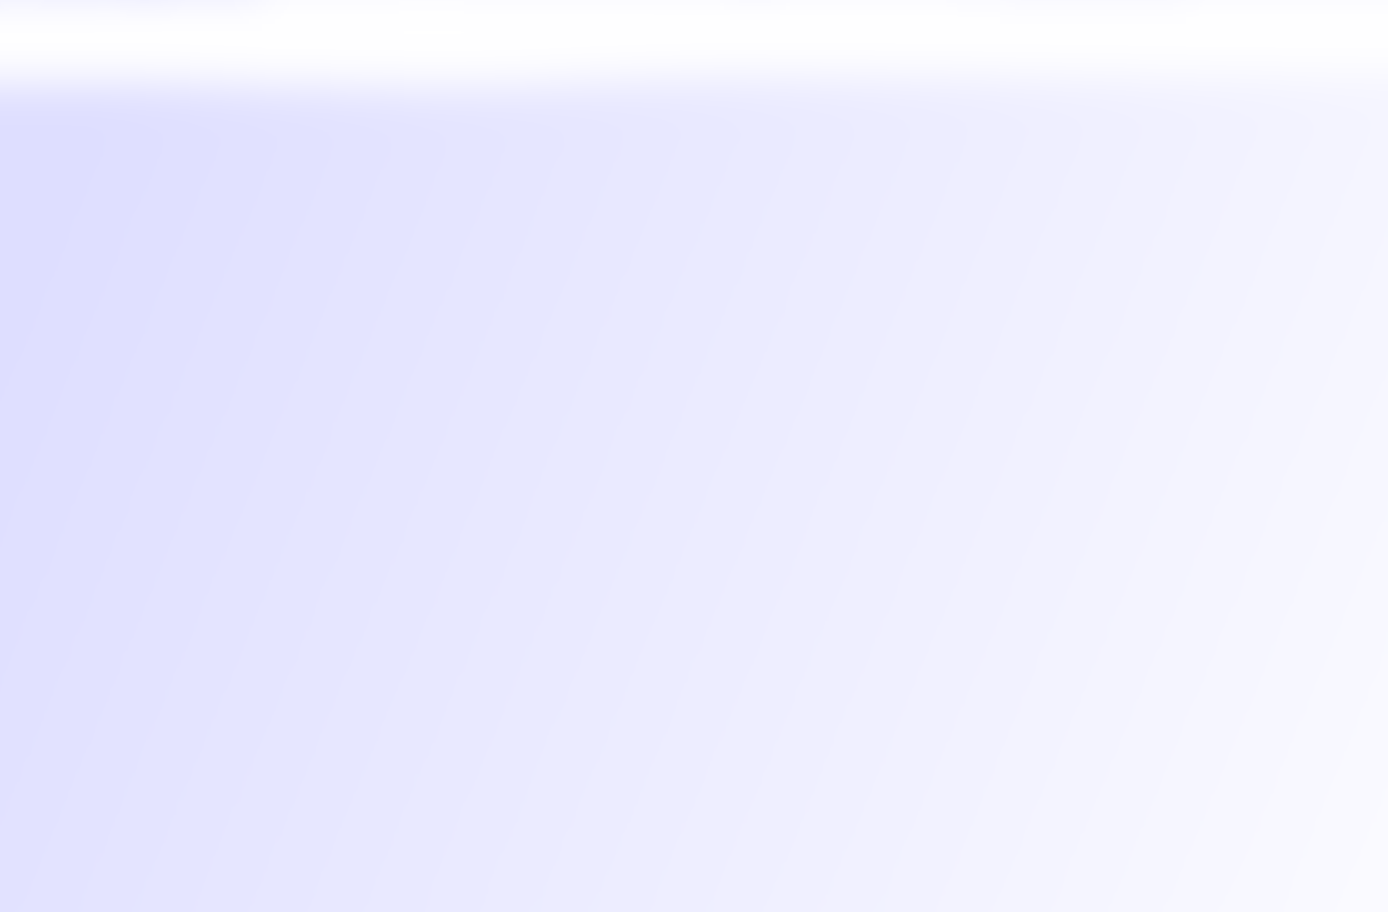
\includegraphics[height=1.1\textheight]{background}};
  \end{tikzpicture}
}
\definecolor{silver}{cmyk}{0,0,0,0.3}
\definecolor{yellow}{cmyk}{0,0,0.9,0.0}
\definecolor{reddishyellow}{cmyk}{0,0.22,1.0,0.0}
\definecolor{black}{cmyk}{0,0,0.0,1.0}
\definecolor{darkYellow}{cmyk}{0,0,1.0,0.5}
\definecolor{darkSilver}{cmyk}{0,0,0,0.1}

\definecolor{lightyellow}{cmyk}{0,0,0.3,0.0}
\definecolor{lighteryellow}{cmyk}{0,0,0.1,0.0}
\definecolor{lighteryellow}{cmyk}{0,0,0.1,0.0}
\definecolor{lightestyellow}{cmyk}{0,0,0.05,0.0}
\begin{poster}{
  % Show grid to help with alignment
  grid=no,
  % Column spacing
  colspacing=0.5em,
  % Color style
  bgColorOne=lighteryellow,
  bgColorTwo=lightestyellow,
  borderColor=reddishyellow,
  headerColorOne=yellow,
  headerColorTwo=reddishyellow,
  headerFontColor=black,
  boxColorOne=lightyellow,
  boxColorTwo=lighteryellow,
  % Format of textbox
  textborder=rectangle,
  % Format of text header
  eyecatcher=no,
  headerborder=open,
  headerheight=0.06\textheight,
  headershape=roundedright,
  headershade=plain,
  headerfont=\large\textsf, %Sans Serif
  boxshade=plain,
%  background=shade-tb,
  background=plain,
  linewidth=2pt
  }
  % Eye Catcher
  {} % No eye catcher for this poster. If an eye catcher is present, the title is centered between eye-catcher and logo.
  % Title
  {\sf %Sans Serif
  %\bf% Serif
  Review of Python-based symbolic mathematics systems and libraries}
  % Authors
  {\sf %Sans Serif
  % Serif
  Mateusz Paprocki$^{1,2}$
  \hspace{3em}
  $^1$ University of Nevada, Reno,
  $^2$ SymPy Development Team
  }
  % University logo
  {{\begin{minipage}{12em}
    \hfill
    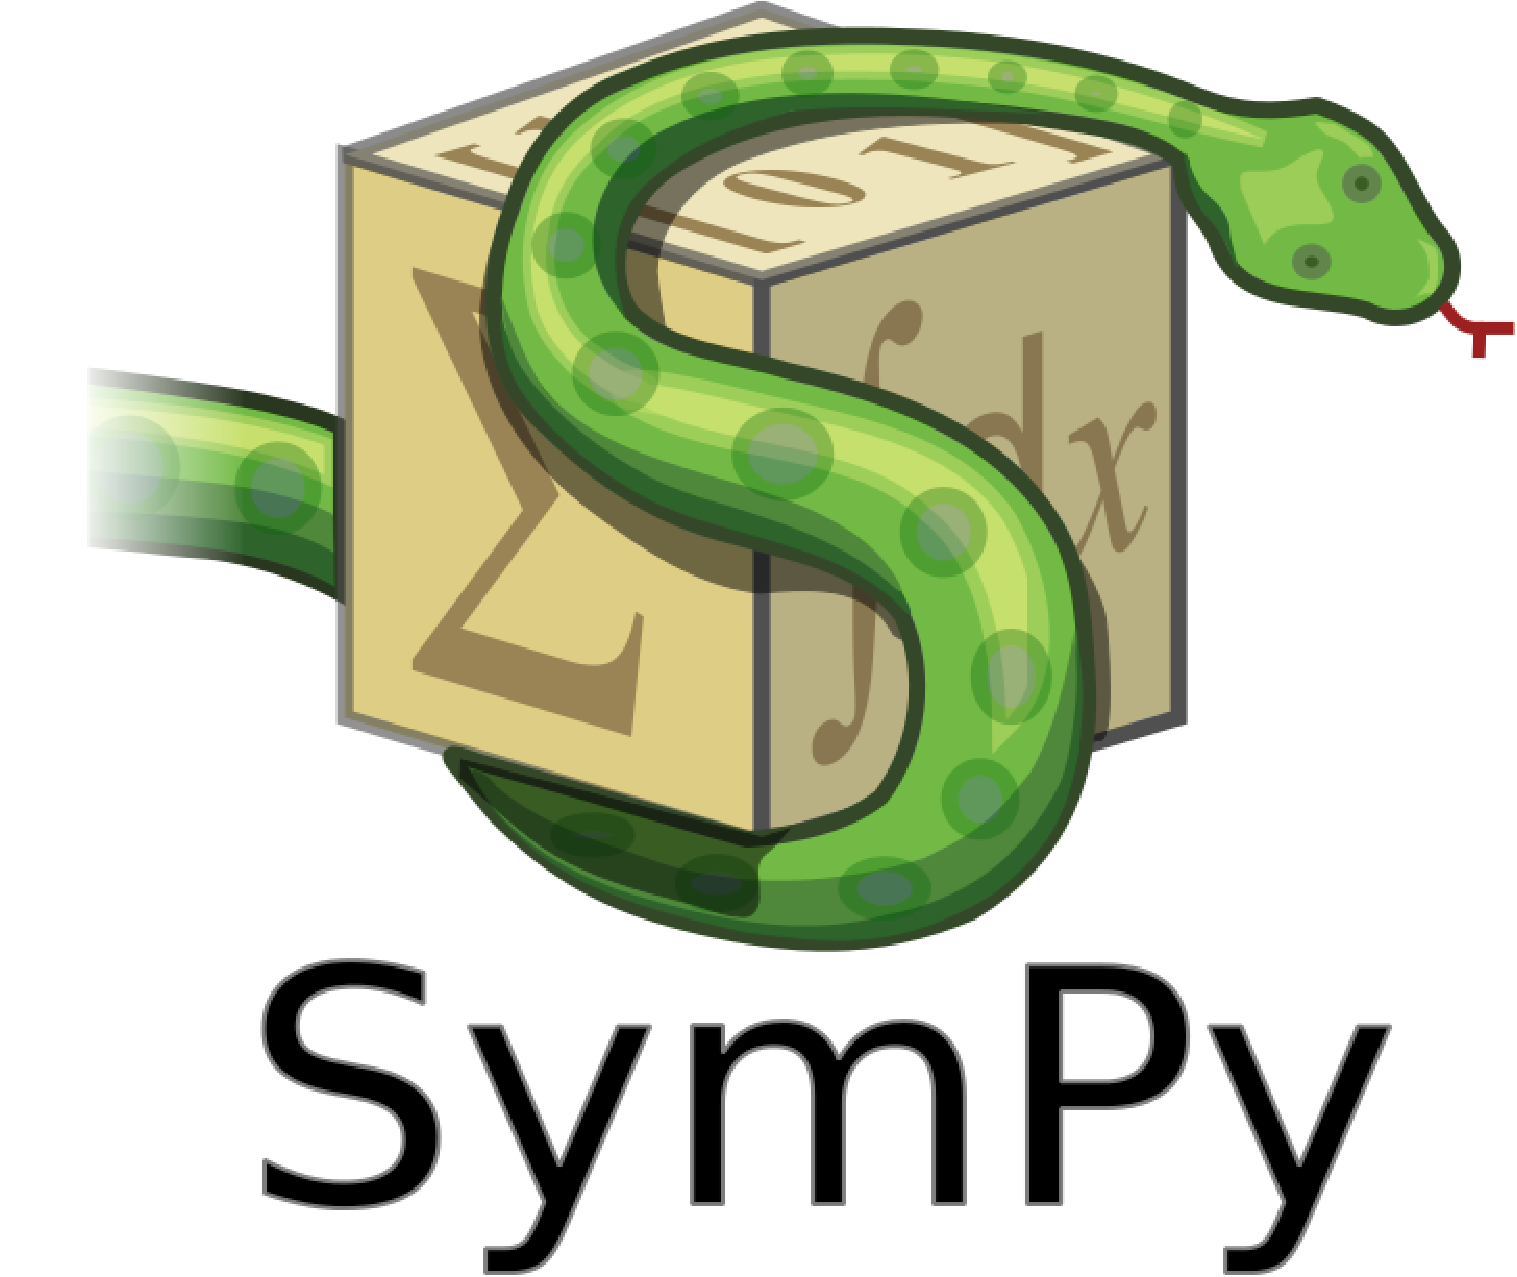
\includegraphics[height=7.0em]{sympy-logo}
  \end{minipage}}
  }

  \tikzstyle{light shaded}=[top color=baposterBGtwo!30!white,bottom color=baposterBGone!30!white,shading=axis,shading angle=30]

  % Width of left inset image
     \newlength{\leftimgwidth}
     \setlength{\leftimgwidth}{0.78em+8.0em}

%%%%%%%%%%%%%%%%%%%%%%%%%%%%%%%%%%%%%%%%%%%%%%%%%%%%%%%%%%%%%%%%%%%%%%%%%%%%%%
%%% Now define the boxes that make up the poster
%%%---------------------------------------------------------------------------
%%% Each box has a name and can be placed absolutely or relatively.
%%% The only inconvenience is that you can only specify a relative position
%%% towards an already declared box. So if you have a box attached to the
%%% bottom, one to the top and a third one which should be in between, you
%%% have to specify the top and bottom boxes before you specify the middle
%%% box.
%%%%%%%%%%%%%%%%%%%%%%%%%%%%%%%%%%%%%%%%%%%%%%%%%%%%%%%%%%%%%%%%%%%%%%%%%%%%%%

%%% {name=hpfem,column=0,below=motivation,span=1,above=bottom}
%%% {name=motivation,column=0,below=contribution}

%%%%%%%%%%%%%%%%%%%%%%%%%%%%%%%%%%%%%%%%%%%%%%%%%%%%%%%%%%%%%%%%%%%%%%%%%%%%%%
\headerbox{Abstract}{name=abstract,column=0,row=0}{
%%%%%%%%%%%%%%%%%%%%%%%%%%%%%%%%%%%%%%%%%%%%%%%%%%%%%%%%%%%%%%%%%%%%%%%%%%%%%%
We compare five Python-based symbolic mathematics systems and libraries:
\textbf{Sage}, \textbf{Swiginac}, \textbf{SymPy}, \textbf{SymPyCore} and
\textbf{Pynac} (in order of first appearance). We would like to make those
systems more familiar to the reader and help answer the question which of
them should be under what circumstances.
}

%%%%%%%%%%%%%%%%%%%%%%%%%%%%%%%%%%%%%%%%%%%%%%%%%%%%%%%%%%%%%%%%%%%%%%%%%%%%%%
\headerbox{Why Python?}{name=why,column=1,span=2,row=0}{
%%%%%%%%%%%%%%%%%%%%%%%%%%%%%%%%%%%%%%%%%%%%%%%%%%%%%%%%%%%%%%%%%%%%%%%%%%%%%%
Python is a modern, general purpose programming language that is easy to
learn but yet very expressive. Almost a complete scientific stack was
created around Python until 2005, which NumPy and SciPy leading the way.
The missing piece of this ecosystem was a system/library for symbolic
mathematics.
}

%%%%%%%%%%%%%%%%%%%%%%%%%%%%%%%%%%%%%%%%%%%%%%%%%%%%%%%%%%%%%%%%%%%%%%%%%%%%%%
\headerbox{Facts}{name=facts,column=0,span=3,below=abstract}{
%%%%%%%%%%%%%%%%%%%%%%%%%%%%%%%%%%%%%%%%%%%%%%%%%%%%%%%%%%%%%%%%%%%%%%%%%%%%%%
\begin{tabular}{l|lllll}
                & Sage                         & Swiginac              & SymPy                  & SymPyCore                   & Pynac              \\\midrule
Website         & www.sagemath.org             & swiginac.berlios.de   & www.sympy.org          & code.google.com/p/sympycore & pynac.sagemath.org \\
Initial release & 24 February 2005             & 25 September 2005     & 11 March 2007          & 29 February 2008            & 8 August 2008      \\
Stable release  & 4.7 (23 May 2011)            & 1.5.1 (15 April 2009) & 0.7.1 (29 July 2011)   & 0.1 (29 February 2008)      & 0.2.2 (9 May 2011) \\
Download size   & 411 MB (Ubuntu 64-bit, lzma) & 100 KB (gzip)         & 3.4 MB (gzip)          & 138 KB (gzip)               & 2.1 MB (bzip2)     \\
Installed size  & 2.4 GB                       & very little           & very little            & very little                 & very little        \\
License         & GNU GPL                      & GNU GPL               & New BSD                & New BSD                     & GNU GPL            \\
Author          & William Stein                & Ola Skavhaug          & Ondrej Certik          & Pearu Peterson              & Burcin Erocal      \\
Contributors    & $>150$                       & $7$                   & $>120$                 & $3$                         & $7$                \\
SCM software    & Mercurial (HG)               & SVN                   & GIT                    & SVN                         & Mercurial (HG)     \\
Languages       & Python, Cython               & C++, Python           & Python                 & Python, C                   & Cython, Python     \\
Web interface   & www.sagenb.org               & none                  & live.sympy.org         & none                        & www.sagenb.org     \\
Influenced by   & Maxima, Magma, ...           & Pyginac               & Swiginac, Maxima       & SymPy                       & Pynac, Swiginac    \\
System origin   & multiple wrappers            & wrappers (Ginac)      & developed from scratch & derivative of SymPy         & wrappers (Ginac)   \\
\end{tabular}
}

%%%%%%%%%%%%%%%%%%%%%%%%%%%%%%%%%%%%%%%%%%%%%%%%%%%%%%%%%%%%%%%%%%%%%%%%%%%%%%
\headerbox{Descriptions}{name=desc,column=0,span=2,below=facts}{
%%%%%%%%%%%%%%%%%%%%%%%%%%%%%%%%%%%%%%%%%%%%%%%%%%%%%%%%%%%%%%%%%%%%%%%%%%%%%%
{\bf Sage} is a free open-source mathematics software system licensed under the GPL. It
combines the power of many existing open-source packages into a common Python-based interface.
\\
{\color{green} Pros:} full scientific stack, very functional, fast
\\
{\color{red} Cons:} very large, not a library, complicated design
\\\\
{\bf Swiginac} is a Python interface to GiNaC, built with SWIG. The aim of swiginac is
to make all the functionality of GiNaC accessible from Python as an extension module.
\\
{\color{green} Pros:} small library, fast
\\
{\color{red} Cons:} not actively developed, written in C++, no community
\\\\
{\bf SymPy} is a Python library for symbolic mathematics. It aims to become a full-featured
computer algebra system (CAS) while keeping the code as simple as possible in order to be
comprehensible and easily extensible. SymPy is written entirely in Python and does not require
any external libraries.
\\
{\color{green} Pros:} small library, pure Python, very functional, embeddable, large community
\\
{\color{red} Cons:} slow, weak documentation
\\\\
{\bf SymPyCore} is inspired by many attempts to implement CAS for Python and it is created
to fix SymPy performance and robustness issues. SymPyCore does not yet have nearly as many
features as SymPy. Our goal is to work on in direction of merging the efforts with the SymPy
project in the future.
\\
{\color{green} Pros:} fast
\\
{\color{red} Cons:} only basic functionality, weak documentation, no community
\\\\
{\bf Pynac} is a derivative of the C++ library GiNaC, which allows manipulation of symbolic
expressions. It currently provides the backend for symbolic expressions in Sage. The main
difference between Pynac and GiNaC is that Pynac relies on Sage to provide the operations
on numerical types, while GiNaC depends on CLN for this purpose.
\\
{\color{green} Pros:} fast, uses Cython for wrapping C++
\\
{\color{red} Cons:} not a standalone library (depends on Sage), only basic functionality
}

%%%%%%%%%%%%%%%%%%%%%%%%%%%%%%%%%%%%%%%%%%%%%%%%%%%%%%%%%%%%%%%%%%%%%%%%%%%%%%
\headerbox{Examples}{name=examples,column=2,span=1,below=facts}{
%%%%%%%%%%%%%%%%%%%%%%%%%%%%%%%%%%%%%%%%%%%%%%%%%%%%%%%%%%%%%%%%%%%%%%%%%%%%%%
{\small
\inputminted{python}{code/sage.py}
\inputminted{python}{code/swiginac.py}
\inputminted{python}{code/sympy.py}
\inputminted{python}{code/sympycore.py}
}
}

%%%%%%%%%%%%%%%%%%%%%%%%%%%%%%%%%%%%%%%%%%%%%%%%%%%%%%%%%%%%%%%%%%%%%%%%%%%%%%
\headerbox{Sage vs. SymPy}{name=sagesympy,column=0,span=2,above=bottom}{
%%%%%%%%%%%%%%%%%%%%%%%%%%%%%%%%%%%%%%%%%%%%%%%%%%%%%%%%%%%%%%%%%%%%%%%%%%%%%%
Sage and SymPy may look very similar, but those are two very different
mathematical systems with completely different internal design,
non-overlapping features sets (e.g. Sage is very good in number theory
abstract algebra, but SymPy has sophisticated pretty printing and code
generation framework) and quite different semantics, e.g.:
\begin{multicols}{2}
    {\small \inputminted{python}{code/sage2.py}}
    {\small \inputminted{python}{code/sympy2.py}}
\end{multicols}
}

%%%%%%%%%%%%%%%%%%%%%%%%%%%%%%%%%%%%%%%%%%%%%%%%%%%%%%%%%%%%%%%%%%%%%%%%%%%%%%
\headerbox{SymPy vs. SymPyCore}{name=sympysympycore,column=2,span=1,below=examples}{
%%%%%%%%%%%%%%%%%%%%%%%%%%%%%%%%%%%%%%%%%%%%%%%%%%%%%%%%%%%%%%%%%%%%%%%%%%%%%%
SymPyCore is a fork of \texttt{sympy.core} module. The project was created
to quickly prototype a new fast symbolic core for SymPy. Over time, SymPyCore
diverged from SymPy and it's unlikely it will be ever merged back.
}

%%%%%%%%%%%%%%%%%%%%%%%%%%%%%%%%%%%%%%%%%%%%%%%%%%%%%%%%%%%%%%%%%%%%%%%%%%%%%%
\headerbox{Pynac vs. Swiginac}{name=pynacswiginac,column=2,span=1,below=sympysympycore}{
%%%%%%%%%%%%%%%%%%%%%%%%%%%%%%%%%%%%%%%%%%%%%%%%%%%%%%%%%%%%%%%%%%%%%%%%%%%%%%
Pynac and Swiginac both wrap Ginac, a C++ library for symbolic computing. Pynac
uses Cython to wrap C++ code and Swiginac uses SWIG library. Both don't wrap the
entire library. Pynac requires Sage for coefficient arithmetics, so you can't use
it a standalone library, as opposed to Swiginac.
}

%%%%%%%%%%%%%%%%%%%%%%%%%%%%%%%%%%%%%%%%%%%%%%%%%%%%%%%%%%%%%%%%%%%%%%%%%%%%%%
\headerbox{Conclusions}{name=conclusions,column=2,span=1,above=bottom}{
%%%%%%%%%%%%%%%%%%%%%%%%%%%%%%%%%%%%%%%%%%%%%%%%%%%%%%%%%%%%%%%%%%%%%%%%%%%%%%
Sage is the most stable and feature complete Python-based mathematics system,
so if you are looking for a ready to use solution that could replace Mathematica
or Maple, then Sage may be the optimal choice. However, Sage is a heavy weight
system with complex internals, so if a light weight, embeddable library is
needed then SymPy may be a better choice. Pynac currently can't be used outside
Sage, so it's usability is very limited.
}

\end{poster}
\end{document}
